\documentclass[margin=1mm]{standalone}
\usepackage{tikz}
\usepackage{pgfplots}
\pgfplotsset{compat=1.16}

% This file contains configuration shared between main file and figures

\usepackage{pifont}
\usepackage{xspace}
\DeclareUnicodeCharacter{2460}{\ding{172}\xspace}
\DeclareUnicodeCharacter{2461}{\ding{173}\xspace}

\usepackage{tikz}

\definecolor{HB9UFblue}{RGB}{0,61,165}
\definecolor{HB9UFred}{HTML}{ED135A}

\newcommand{\Ohm}{$\Omega$\xspace}


\newcommand{\uline}[1]{%
  \tikz[baseline=(todotted.base)]{
      \node[inner sep=1pt,outer sep=0pt] (todotted) {#1};
      \draw[color=HB9UFblue,thick] (todotted.south west) -- (todotted.south east);
  }%
}%
                           
\newcommand{\udash}[1]{%
  \tikz[baseline=(todotted.base)]{
      \node[inner sep=1pt,outer sep=0pt] (todotted) {#1};
      \draw[dashed,color=HB9UFred,thick] (todotted.south west) -- (todotted.south east);
  }%
}%


\begin{document}
    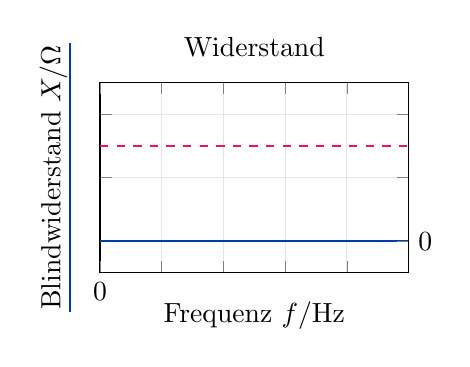
\begin{tikzpicture}
        \begin{axis}[
            title = {Widerstand},
            xmin=0, xmax=10,
            ymin=-100,ymax=500,
            grid=both,
            xlabel={Frequenz $f$/Hz},
            ylabel={\uline{Blindwiderstand $X/\Omega$}},
            xticklabels={},
            yticklabels={},
            ytick = {-400,-200,0,200,400},
            height=4cm,
            width=5.5cm,
            major grid style={black!10}
        ]
        \addplot [mark=none,samples=100,domain=0:10,color=HB9UFblue,thick] {0};
        \end{axis}
        \begin{axis}[
            xmin=0, xmax=10,
            ymin=-100,ymax=500,
            grid=none,
            separate axis lines,
            ylabel style = {align=center},
            ticks=none,
            xmajorticks=true,
            xminorticks=false,
            ymajorticks=true,
            yminorticks=false,
            scaled ticks=false,
            xtick = {0},
            ytick = {0},
            axis y line*=right,
            height=4cm,
            width=5.5cm,
            major grid style={black!10}
        ]
        \addplot [mark=none,samples=100,domain=0:10,color=HB9UFred,dashed,thick] {300};
        \end{axis}
    \end{tikzpicture}\hfill
    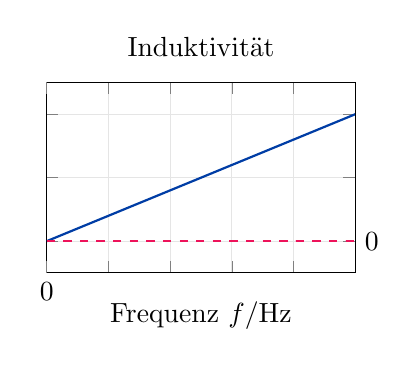
\begin{tikzpicture}
        \begin{axis}[
            title = {Induktivität},
            xmin=0, xmax=10,
            ymin=-100,ymax=500,
            grid=both,
            xlabel={Frequenz $f$/Hz},
            xticklabels={},
            yticklabels={},
            ytick = {-400,-200,0,200,400},
            height=4cm,
            width=5.5cm,
            major grid style={black!10}
        ]
        \addplot [mark=none,samples=100,domain=0:10,color=HB9UFblue,thick] {40*x};
        \end{axis}
        \begin{axis}[
            xmin=0, xmax=10,
            ymin=-100,ymax=500,
            grid=none,
            separate axis lines,
            ylabel style = {align=center},
            ticks=none,
            xmajorticks=true,
            xminorticks=false,
            ymajorticks=true,
            yminorticks=false,
            scaled ticks=false,
            xtick = {0},
            ytick = {0},
            axis y line*=right,
            height=4cm,
            width=5.5cm,
            major grid style={black!10}
        ]
        \addplot [mark=none,samples=100,domain=0:10,color=HB9UFred,dashed,thick] {0};
        \end{axis}
    \end{tikzpicture}\hfill
    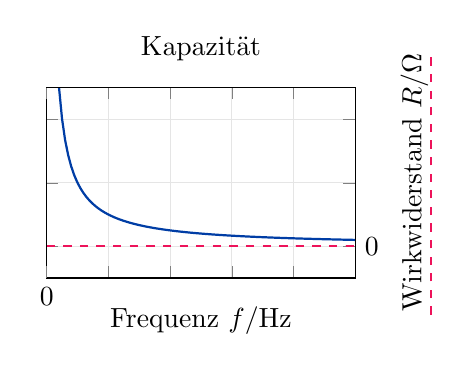
\begin{tikzpicture}
        \begin{axis}[
            title = {Kapazität},
            xmin=0, xmax=10,
            ymin=-100,ymax=500,
            grid=both,
            xlabel={Frequenz $f$/Hz},
            xticklabels={},
            yticklabels={},
            ytick = {0,200,400},
            height=4cm,
            width=5.5cm,
            major grid style={black!10}
        ]
        \addplot [mark=none,samples=100,domain=0.2:10,color=HB9UFblue,thick] {200/x};
        \end{axis}
        \begin{axis}[
            xmin=0, xmax=10,
            ymin=-100,ymax=500,
            grid=none,
            separate axis lines,
            ylabel style = {align=center},
            ylabel={\udash{Wirkwiderstand $R/\Omega$}},
            ticks=none,
            xmajorticks=true,
            xminorticks=false,
            ymajorticks=true,
            yminorticks=false,
            scaled ticks=false,
            xtick = {0},
            ytick = {0},
            axis y line*=right,
            height=4cm,
            width=5.5cm,
            major grid style={black!10}
        ]
        \addplot [mark=none,samples=100,domain=0:10,color=HB9UFred,dashed,thick] {0};
        \end{axis}
    \end{tikzpicture}
\end{document}
